\documentclass[]{article}
\newcommand{\FileDepth}{../../..}
\usepackage[letterpaper, landscape, margin=0.5cm]{geometry}
\usepackage[T1]{fontenc}
\usepackage{textcomp}%Not strictly necessary, but gives \textmu command for "micro."
\usepackage{fancyhdr}
\usepackage{amsmath}
\usepackage{amssymb}
\usepackage{graphicx}
\usepackage{xcolor}
\usepackage{tikz}
\usetikzlibrary{calc}
\usepackage[shortlabels]{enumitem}
\usepackage{multicol}
\usepackage{vwcol}
\usepackage{hyperref}
\usepackage{wrapfig}
%opening
\newcommand{\SecType}{L}
\newcommand{\Week}{17}
\title{PH 211 Lecture \Week}
\author{Benjamin Bauml}
\date{Summer 2024}

\newcommand{\Purpose}{4}
\newcommand{\DefOnly}{0}

% Version 2024-06-14
% Changes
% 2024-02-21 Added xstring package to enable smooth implementation of new \ModePage command.
% 2024-04-27 Set up to split activities and formatting aspects into separate files. Removed dependence on xcomment. Added an automatic counter to number the activities in a problem set.
% 2024-05-19 Revised old format for \TeachingTips command, which did not support \DefOnly.
% 2024-06-14 Added Repurpose environment to allow mixing of different purpose levels in the same document.
\usepackage{tcolorbox}
\usepackage{xstring}
% You will want the following four lines in your document (the last two uncommented):
% For Assignment, leave Purpose as 1. For Worksheet, set to 2. For Student Solution, set to 3. For Teacher Solution, set to 4.
% If you want keep the pieces from being called manually, set DefOnly to 0.
%\newcommand{\Purpose}{4}
%\newcommand{\DefOnly}{1}
\newcommand{\Exclusion}{0}
\newcommand{\PageTurn}{0}
\newcommand{\GrayProb}{0}
\newcommand{\Tipsy}{0}

% Assignment
\if\Purpose1
\renewcommand{\Exclusion}{1}
\fi
% Worksheet
\if\Purpose2
\renewcommand{\Exclusion}{1}
\renewcommand{\PageTurn}{1}
\fi
% Student Solution
\if\Purpose3
\renewcommand{\PageTurn}{1}
\renewcommand{\GrayProb}{1}
\fi
% Teaching Copy
\if\Purpose4
\renewcommand{\PageTurn}{1}
\renewcommand{\GrayProb}{1}
\renewcommand{\Tipsy}{1}
\fi

\newenvironment{Repurpose}[1]{
\renewcommand{\Purpose}{#1}
\renewcommand{\Exclusion}{0}
\renewcommand{\PageTurn}{0}
\renewcommand{\GrayProb}{0}
\renewcommand{\Tipsy}{0}
% Assignment
\if\Purpose1
\renewcommand{\Exclusion}{1}
\fi
% Worksheet
\if\Purpose2
\renewcommand{\Exclusion}{1}
\renewcommand{\PageTurn}{1}
\fi
% Student Solution
\if\Purpose3
\renewcommand{\PageTurn}{1}
\renewcommand{\GrayProb}{1}
\fi
% Teaching Copy
\if\Purpose4
\renewcommand{\PageTurn}{1}
\renewcommand{\GrayProb}{1}
\renewcommand{\Tipsy}{1}
\fi
}{}

\def \NewQ {0}
\def \PForce {0}
\newcommand{\MaybePage}[1]{
	\def \PForce {#1}
	\if\PForce1
	\newpage
	\else
	\if\NewQ0
	\gdef \NewQ {\PageTurn}
	\else
	\newpage
	\fi
	\fi
}

\newcommand{\ModePage}[1]{
	\IfSubStr{#1}{\Purpose}{\newpage}{}
}

\newcounter{ActNumber}
\setcounter{ActNumber}{0}

\newcommand{\Problem}[4][0]{%The first argument is optional, and if it is set to 1, the \newpage will be forced. The second argument is the name of the activity, the third is the command the activity is stored as, and the fourth is the actual problem statement.
\newcommand{#3}{
\MaybePage{#1}
\addtocounter{ActNumber}{1}
\section*{\SecType\Week-\theActNumber: #2}
\if\GrayProb1
\begin{tcolorbox}[colback=lightgray,colframe=lightgray,sharp corners,boxsep=1pt,left=0pt,right=0pt,top=0pt,bottom=0pt,after skip=2pt]
\else
\begin{tcolorbox}[colback=white,colframe=white,sharp corners,boxsep=1pt,left=0pt,right=0pt,top=0pt,bottom=0pt,after skip=2pt]
\fi
#4
\end{tcolorbox}\noindent
}
\if\DefOnly0
\else
#3
\fi
}
	
\newcommand{\ProblemSub}[3][0]{%The first argument is optional, and if a string of numbers is entered into it, it will force a \newpage in any \Purpose that shows up in the string. For example, "13" would lead to the newpage being forced in modes 1 and 3. The second is the command the activity is stored as, and the third is the actual problem statement.
\newcommand{#2}{
\ModePage{#1}
\if\GrayProb1
\begin{tcolorbox}[colback=lightgray,colframe=lightgray,sharp corners,boxsep=1pt,left=0pt,right=0pt,top=0pt,bottom=0pt,after skip=2pt]
\else
\begin{tcolorbox}[colback=white,colframe=white,sharp corners,boxsep=1pt,left=0pt,right=0pt,top=0pt,bottom=0pt,after skip=2pt]
\fi
#3
\end{tcolorbox}\noindent
}
\if\DefOnly0
\else
#2
\fi
}
		
\newcommand{\Solution}[2]{%The first argument is the command the solution is stored as, and the second is the actual solution.
\newcommand{#1}{
\if\Exclusion0
#2
\fi
}
\if\DefOnly0
\else
#1
\fi
}
		
\newcommand{\ProblemFig}[2]{%The first argument is the command the figure is stored as, and the second is the actual figure.
\newcommand{#1}{
\begin{figure}[h]
#2
\end{figure}
}
\if\DefOnly0
\else
#1
\fi
}

\newcommand{\TeachingTips}[2]{%The first argument is the command the tip is stored as, and the second is the actual tip.
\newcommand{#1}{
\if\Tipsy1
\begin{tcolorbox}[colback=lightgray,colframe=black]
#2
\end{tcolorbox}
\fi
}
\if\DefOnly0
\else
#1
\fi
}
\usepackage[absolute]{textpos}
% This package relies on Assignment Format 2024-06-14 or later to work. It is recommended that the Purpose and DefOnly commands be given as such:
%\newcommand{\Purpose}{4}
%\newcommand{\DefOnly}{0}
% Activities need to be entered outside of the TeacherMargin and PresentSpace environments, otherwise they will be defined only locally. They can even go in the preamble.
\newenvironment{TeacherMargin}{\begin{textblock*}{10.8cm}(0.5cm,0.5cm)
\small}{\end{textblock*}
\hspace{0.1cm}}
\newenvironment{PresentSpace}{\begin{textblock*}{0.3cm}(26.85cm,9.35cm)
--
\end{textblock*}
\begin{textblock*}{0.3cm}(26.85cm,18.7cm)
--
\end{textblock*}
\begin{textblock*}{0.3cm}(26.85cm,12.24cm)
	--
\end{textblock*}
\begin{textblock*}{15.6cm}(11.8cm,0.5cm)
\begin{Repurpose}{1}
\Large}{\end{Repurpose}
\end{textblock*}
\hspace{0.1cm}}

%\newcommand{\FBDaxes}[3]{
	\begin{scope}[shift={(#1)},rotate=#2]
		% x-axis
		\draw[thick,->] (-2,0) -- (2,0);
		\node[anchor=west] at (2,0) {$x$};
		% y-axis
		\draw[thick,->] (0,-2) -- (0,2);
		\node[anchor=west] at (0,2) {$y$};
		\coordinate (#3) at (0,0);
	\end{scope}
}
\newcommand{\FBDvectorMA}[4]{
	\begin{scope}[shift={(#1)}]
		\coordinate (#4tip) at ({#2*cos(#3)},{#2*sin(#3)});
		\draw[ultra thick,blue,->] (#1) -- (#4tip);
	\end{scope}
}
\newcommand{\FBDvectorXY}[3]{
	\begin{scope}[shift={(#1)}]
		\coordinate (#3tip) at (#2);
		\draw[ultra thick,blue,->] (0,0) -- (#3tip);
	\end{scope}
}
\newcommand{\FBDdot}[1]{
	\filldraw[black] (#1) circle (3pt);
}
%\newcommand{\MVec}[3][0]{%Creates a momentum vector of length #3 centered at #2 and rotated #1 degrees counterclockwise.
	\begin{scope}[rotate=#1,shift={(#2)}]
		\draw[->,thick] ({-#3/2},0) -- ({#3/2},0);
	\end{scope}
}
\newcommand{\MDot}[1]{%Creates a dot at #1 to represent a zero vector.
	\filldraw (#1) circle (1pt);
}
\newcommand{\MVDRows}[2][4.5]{%Creates the rows (initial, delta, final) of a momentum vector diagram. The optional argument determines the width of the table, and defaults to a good length for three columns (two objects and the total system). The non-optional argument gives a coordinate name (not displayed) to the diagram.
	\begin{scope}
		%\draw[thick] (0,5.5) -- (0,0);
		\draw[thick] (-1,4.5) -- (#1,4.5);
		\node at (-0.5,3.75) {$\vec{p}_{i}$};
		\draw[thick] (-1,3) -- (#1,3);
		\node at (-0.5,2.25) {$\Delta\vec{p}$};
		\draw[thick] (-1,1.5) -- (#1,1.5);
		\node at (-0.5,0.75) {$\vec{p}_{f}$};
		\coordinate (#2) at (0,5);
	\end{scope}
}
\newcommand{\MVDCol}[4][0.75]{%Creates a column for an object in a momentum vector diagram. The first (non-optional) argument is the coordinate name (not displayed) of the column, while the second is the displayed column header. The first argument also names the three entries down the column. The third argument anchors the column, so it should either be the coordinate name of the MVD (for the first column) or the coordinate name of the previous column. The optional argument indicates how far the center of the column should be from the previous column's edge, and defaults to 0.75
	\begin{scope}[shift={(#4)}]
		\node at (#1,0) {#3};
		%\draw[thick] ({#1*2},0.5) -- ({#1*2},-5);
		\draw[thick] (0,0.5) -- (0,-5);
		\coordinate (#2init) at (#1,-1.25);
		\coordinate (#2delt) at (#1,-2.75);
		\coordinate (#2fin) at (#1,-4.25);
		\coordinate (#2) at ({#1*2},0);
	\end{scope}
}

%\input{\FileDepth/Activities/Activity_One/Activity_One.tex}
%\input{\FileDepth/Activities/Activity_Two/Activity_Two.tex}

\begin{document}
\begin{TeacherMargin}

\end{TeacherMargin}
\begin{PresentSpace}
\begin{center}
	\huge Lecture \Week: Potential Energy
\end{center}
\vspace{0.5cm}
\underline{Warm-Up Activity} \\
Question?
%\begin{multicols}{2}
\begin{enumerate}[(A)]
	\item Answer?
\end{enumerate}
%\end{multicols}
\end{PresentSpace}
\newpage
\begin{TeacherMargin}

\end{TeacherMargin}
\begin{PresentSpace}
\vspace{-10pt}
\section*{A Deeper Model for Interactions}
\vspace{-10pt}
\begin{itemize}
	\item Quantities
	\begin{itemize}
		\item Energy \qquad \qquad \qquad \quad \ \ $E$
		\item Work \qquad \qquad \qquad \quad \ \ \ \ $W = \int_{r_{i}}^{r_{f}}\vec{F}\cdot d\vec{r}$
		\item Kinetic Energy \qquad \qquad $K=\frac{1}{2}mv^{2}$
	\end{itemize}
	\item Laws
	\begin{itemize}
		\item Work-energy theorem \quad $W_{\text{net,ext}} = \Delta E_{\text{total}}$
	\end{itemize}
\end{itemize}
\end{PresentSpace}
\newpage
\begin{TeacherMargin}

\end{TeacherMargin}
\begin{PresentSpace}
\vspace{-10pt}
\section*{Potential Energy}
\vspace{-10pt}
\begin{itemize}
	\item Potential energy is present when there is an \textit{internal} interaction between objects within a system.
	\item How do we figure out how much potential energy something has?
	\begin{itemize}
		\item We can look at the work that the internal interaction would have done if it were external.
	\end{itemize}
	\item For special kinds of internal forces (called \textit{conservative} forces):
	\[
	\Delta U = -W_{\text{internal}}
	\]
\end{itemize}
\end{PresentSpace}
\newpage
\begin{TeacherMargin}
\begin{center}
	\scalebox{0.75}{
	\begin{tabular}{|c|c|c|}
		\hline
		Questions & \parbox{2.5cm}{\centering \phantom{\tiny Blank} \\ System 1: \\ Tennis Ball \small \\ \phantom{Blank}} & \parbox{4.5cm}{\centering System 2: \\ Tennis Ball + Earth} \\
		\hline\hline
		\parbox{4cm}{\centering\phantom{\small Blank} \\ External forces? \small \\ \phantom{Blank}} & Gravity & None \\ \hline
		\parbox{4cm}{\centering\phantom{\small Blank} \\ $W_{\text{net,ext}}$ \small \\ \phantom{Blank}} & $+mgh$ & 0 \\ \hline
		\parbox{4cm}{\centering\phantom{\small Blank} \\ $\Delta E_{\text{total}}$ \small \\ \phantom{Blank}} & $+mgh$ & 0 \\ \hline
		\parbox{4cm}{\centering\vspace{6pt} What kinds of E are there and how have they changed?\vspace{6pt}} & Kinetic energy increases. & \parbox{4cm}{Kinetic energy increases. Potential energy decreases.} \\ \hline
	\end{tabular}
	}
\end{center}
\end{TeacherMargin}
\begin{PresentSpace}
\vspace{-10pt}
\section*{L\Week-1: Gravitational Potential Energy}
\vspace{-10pt}
You drop a tennis ball (mass $m$) off the top of a tall building (height $h$).
\begin{center}
\begin{tabular}{|c|c|c|}
	\hline
	Questions & \parbox{2.5cm}{\centering \phantom{\tiny Blank} \\ System 1: \\ Tennis Ball \small \\ \phantom{Blank}} & \parbox{4.5cm}{\centering System 2: \\ Tennis Ball + Earth} \\
	\hline\hline
	\parbox{4cm}{\centering\phantom{\small Blank} \\ External forces? \small \\ \phantom{Blank}} & & \\ \hline
	\parbox{4cm}{\centering\phantom{\small Blank} \\ $W_{\text{net,ext}}$ \small \\ \phantom{Blank}} & & \\ \hline
	\parbox{4cm}{\centering\phantom{\small Blank} \\ $\Delta E_{\text{total}}$ \small \\ \phantom{Blank}} & & \\ \hline
	\parbox{4cm}{\centering\vspace{6pt} What kinds of E are there and how have they changed?\vspace{6pt}} & & \\ \hline
\end{tabular}
\end{center}
\end{PresentSpace}
\newpage
\begin{TeacherMargin}

\end{TeacherMargin}
\begin{PresentSpace}
\vspace{-10pt}
\section*{Gravitational Potential Energy}
\vspace{-10pt}
When a mass $m$ in a system changes its height by an amount $\Delta h$:
\begin{enumerate}[(A)]
	\item If we don't include the Earth in the system, then the Earth does work on the system equal to
	\[
	W_{g} = -mg\Delta h.
	\]
	This changes the total energy of the system.
	\item If we include the Earth in the system, then the potential energy of the system changes by an amount
	\[
	\Delta U_{g} = mg\Delta h.
	\]
	This does not change the total energy of the system.
\end{enumerate}
\end{PresentSpace}
\newpage
\begin{TeacherMargin}
\noindent\textbf{Other Kinds of Energy} \\
In PH 212, you will work with rotational kinetic energy and the energy carried by different types of waves, and in PH 213, you will work with electric potential energy. \\

\noindent There are other kinds of energy. To name just a few, you might deal with chemical energy in some situations, or perhaps you could think about the energy stored in pressurized gas (thermodynamics will teach you a lot about how changes in pressure and volume will affect the temperature of a gas).
\end{TeacherMargin}
\begin{PresentSpace}
\vspace{-10pt}
\section*{A Deeper Model for Interactions}
\vspace{-10pt}
\begin{itemize}
	\item Quantities
	\begin{itemize}
		\item Energy \qquad \qquad \qquad \quad \ \ $E$
		\item Work \qquad \qquad \qquad \quad \ \ \ \ $W = \int_{r_{i}}^{r_{f}}\vec{F}\cdot d\vec{r}$
		\item Kinetic Energy \qquad \qquad $K=\frac{1}{2}mv^{2}$
		\item Potential Energy \qquad \quad \ $U=$ depends on interaction \\
		You have to tell everyone where zero $PE$ is!
		\begin{itemize}
			\item Gravity \qquad $U_{g} = mgy$
			\item Spring \qquad \ $U_{sp} = \frac{1}{2}kx^{2}$
		\end{itemize}
	\end{itemize}
	\item Laws
	\begin{itemize}
		\item Work-energy theorem \quad $W_{\text{net,ext}} = \Delta E_{\text{total}}$
	\end{itemize}
\end{itemize}
\end{PresentSpace}
\newpage
\begin{TeacherMargin}
\noindent (B) 600 J \\
The displacement is squared ($U_{sp}=\frac{1}{2}kx^{2}$), so it doesn't matter if it is positive or negative. The same amount of stretch or compression stores the same amount of energy.
\end{TeacherMargin}
\begin{PresentSpace}
\vspace{-10pt}
\section*{L\Week-2: Stretch vs. Compression}
\vspace{-10pt}
\begin{itemize}
	\item A spring's potential energy is 0 J at $x=0$ (equilibrium).
	\item When you stretch the spring to the right ($x=+3$ cm), the spring's potential energy is 600 J.
	\item What is the spring's potential energy when you compress the spring to the left ($x=-3cm$)?
	\begin{enumerate}[(A)]
		\item 1200 J
		\item 600 J
		\item 0 J
		\item $-600$ J
		\item $-1200$ J
	\end{enumerate}
\end{itemize}
\end{PresentSpace}
\newpage
\begin{TeacherMargin}
\noindent (D) $-$600 J \\
If you can change to a lower height, you can always decrease gravitational potential energy. There is always more energy to access, even if you start at zero. The choice of zero is arbitrary; the change in potential energy is what matters.
\end{TeacherMargin}
\begin{PresentSpace}
\vspace{-10pt}
\section*{L\Week-3: Second Floor vs. Basement}
\vspace{-10pt}
\begin{itemize}
	\item An object's gravitational potential energy with the Earth is 0 J on the \textbf{first floor}.
	\item On the \textbf{second floor}, 3 meters above the first floor, the gravitational potential energy is 600 J.
	\item What is the gravitational potential energy when the object is in the basement (3 meters underground)?
	\begin{enumerate}[(A)]
		\item 1200 J
		\item 600 J
		\item 0 J
		\item $-600$ J
		\item $-1200$ J
	\end{enumerate}
\end{itemize}
\end{PresentSpace}
\newpage
\begin{TeacherMargin}

\end{TeacherMargin}
\begin{PresentSpace}
\vspace{-10pt}
\section*{Solving Problems with Energy}
\vspace{-10pt}
\begin{itemize}
	\item The energy of a system depends on:
	\begin{itemize}
		\item \textit{where} each object is located (potential),
		\item \textit{how fast} each object is moving (kinetic).
	\end{itemize}
	\item The \textbf{change} in a system's energy is often easy to calculate.
\end{itemize}
\end{PresentSpace}
\newpage
\begin{TeacherMargin}
\noindent \textbf{System} \\
Your system should be you and the Earth. If the Earth is outside of our system, then gravity does work on you. We can solve the problem this way, but that is not the method of conservation of energy. By putting you and the Earth in the system, there is no work done, and you and the Earth share gravitational potential energy. \\

\noindent It can be very helpful to organize our energies into a table. Each row is a different point in time, and each column is a type of energy in the system, written as a symbolic equation. The right column is the total energy, each entry of which is obtained by summing all of the different energy equations in that row.
\begin{center}
\Large
\begin{tabular}{|c|c|c||c|}
	\hline
	& $K$ & $U_{g}$ & $E_{\text{total}}$ \\ \hline
	Initial & 0 & $mgh$ & $mgh$ \\ \hline
	Final & $\frac{1}{2}mv^{2}$ & 0 & $\frac{1}{2}mv^{2}$ \\ \hline
\end{tabular}
\end{center}
The work energy theorem tells us that
\begin{align*}
	\Delta E & = W_{\text{net,ext}} \\
	E_{f}-E_{i} & = 0 \\
	E_{f} & = E_{i}.
\end{align*}
As such, if we know there is no work done between two times in our table, we can set the total energy entries of those rows equal to each other. In particular:
\begin{align*}
	\frac{1}{2}mv^{2} & = mgh \\
	v & = \sqrt{2gh}.
\end{align*}
Note that the angle of the waterslide doesn't matter! The change in height is important, but how exactly we get from the top to the bottom doesn't matter. This is an aspect of gravity being a conservative force.
\end{TeacherMargin}
\begin{PresentSpace}
\vspace{-10pt}
\section*{L\Week-4: Down a Waterslide}
\vspace{-10pt}
\begin{itemize}
	\item You (mass $m$) slide down a frictionless waterslide (height $h$) that makes an angle $\theta$.
	\item How fast are you moving at the bottom of the waterslide?
	\begin{itemize}
		\item What system do you want to choose?
		\item What kinds of energy do we have?
	\end{itemize}
\end{itemize}
\end{PresentSpace}
\newpage
\begin{TeacherMargin}
\noindent \textbf{System} \\
The system should be the spring and the rock. This makes the spring force internal, so we can use spring potential energy instead of work done by the spring.
\begin{center}
	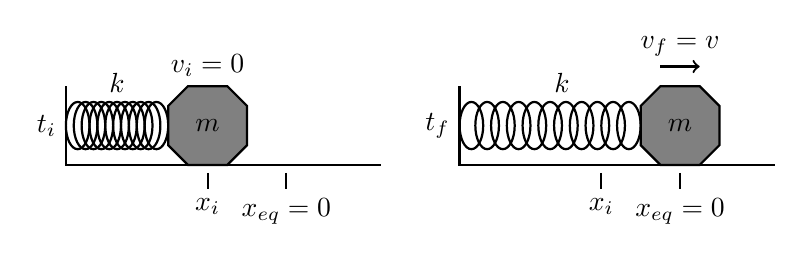
\begin{tikzpicture}
		\begin{scope}
			\node[anchor=east] at (0,0.5) {$t_{i}$};
			\draw[thick] (0,1) -- (0,0) -- (4,0);
			\foreach \s in {0,1,2,3,4,5,6,7,8,9,10}
				\draw[thick] (\s*0.1+0.15,0.5) circle (0.15 and 0.3);
			\node[anchor=south] at (0.65,0.8) {$k$};
			\draw[thick,color=black,fill=gray,shift={(1.3,0)}] (0,0.5) -- (0,0.75) -- (0.25,1) -- (0.75,1) -- (1,0.75) -- (1,0.25) -- (0.75,0) -- (0.25,0) -- (0,0.25) -- cycle;
			\node at (1.8,0.5) {$m$};
			\node[anchor=south] at (1.8,1) {$v_{i}=0$};
			\draw[thick] (1.8,-0.1) -- (1.8,-0.3) node[anchor=north] {$x_{i}$};
			\draw[thick] (2.8,-0.1) -- (2.8,-0.3) node[anchor=north] {$x_{eq}=0$};
		\end{scope}
		\begin{scope}[shift={(5,0)}]
			\node[anchor=east] at (0,0.5) {$t_{f}$};
			\draw[thick] (0,1) -- (0,0) -- (4,0);
			\foreach \s in {0,1,2,3,4,5,6,7,8,9,10}
				\draw[thick] (\s*0.2+0.15,0.5) circle (0.15 and 0.3);
			\node[anchor=south] at (1.3,0.8) {$k$};
			\draw[thick,color=black,fill=gray,shift={(2.3,0)}] (0,0.5) -- (0,0.75) -- (0.25,1) -- (0.75,1) -- (1,0.75) -- (1,0.25) -- (0.75,0) -- (0.25,0) -- (0,0.25) -- cycle;
			\node at (2.8,0.5) {$m$};
			\draw[thick,->,shift={(2.3,0)}] (0.25,1.25) -- (0.5,1.25) -- (0.75,1.25);
			\node[anchor=south] at (2.8,1.25) {$v_{f}=v$};
			\draw[thick] (1.8,-0.1) -- (1.8,-0.3) node[anchor=north] {$x_{i}$};
			\draw[thick] (2.8,-0.1) -- (2.8,-0.3) node[anchor=north] {$x_{eq}=0$};
		\end{scope}
	\end{tikzpicture}
	\Large
	\begin{tabular}{|c|c|c||c|}
		\hline
		& $K$ & $U_{sp}$ & $E_{\text{total}}$ \\ \hline
		$t_{i}$ & 0 & $\frac{1}{2}kx_{i}^{2}$ & $\frac{1}{2}kx_{i}^{2}$ \\ \hline
		$t_{f}$ & $\frac{1}{2}mv^{2}$ & 0 & $\frac{1}{2}mv^{2}$ \\ \hline
	\end{tabular}
\end{center}
There is no external work being done on this system, so $\Delta E_{\text{total}}=0$ by the work-energy theorem. As such, the total energy is conserved, and $E_{f} = E_{i}$:
\begin{align*}
	\frac{1}{2}mv^{2} & = \frac{1}{2}kx_{i}^{2} \\
	v^{2} & = \frac{k}{m}x_{i}^{2} \\
	v & = x_{i}\sqrt{\frac{k}{m}}.
\end{align*}
\end{TeacherMargin}
\begin{PresentSpace}
\vspace{-10pt}
\section*{L\Week-5: Rock with a Spring}
\vspace{-10pt}
\begin{itemize}
	\item A rock (mass $m$) is compressing a horizontal spring with constant $k$ by an amount $x_{i}$.
	\item If you release the rock from rest, how fast is the rock moving when the spring returns to equilibrium?
	\begin{itemize}
		\item What system do you want to choose?
		\item What kinds of energy do we have?
		\item Draw a diagram to help!
		\item Find the speed of the rock.
	\end{itemize}
\end{itemize}
\end{PresentSpace}
\newpage
\begin{TeacherMargin}

\end{TeacherMargin}
\begin{PresentSpace}
\vspace{-10pt}
\section*{Solving Problems with Energy}
\vspace{-10pt}
\begin{itemize}
	\item The \textbf{change} in a system's energy is often easy to calculate.
	\begin{itemize}
		\item Choose a system.
		\item Identify all forms of energy.
		\item Draw energy bar diagrams.
		\begin{itemize}
			\item A simple, descriptive before-and-after sketch is also good for setting up the problem.
			\item An energy bar diagram helps you translate from the positions and velocities of the objects into what you expect the energies to be doing over time.
		\end{itemize}
		\item Identify each energy symbolically.
		\begin{itemize}
			\item Organize them in a table!
		\end{itemize}
	\end{itemize}
\end{itemize}
\end{PresentSpace}
\newpage
\begin{TeacherMargin}
	
\end{TeacherMargin}
\begin{PresentSpace}
\section*{Main Ideas}
\begin{itemize}
	\item We can solve physics problems from an \textit{energy approach} instead of from a \textit{force approach}.
\end{itemize}
\end{PresentSpace}
\end{document}